\chapter{Summary}
\textbf{Figure \texttt{10\_27a}}: The method we used to solve this problem was good and use of any other algorithm would have been the same.
\\
\\
\textbf{Figure \texttt{10\_27d}}: It was a good strategy to divide the image into blocks and use Otsu’s segmentation on it. We did have a small amount of error which could have been avoided using moving window method.
\\
\\
\textbf{Figure \texttt{group\_of\_coins}}: For this image we used Otsus method and the we eroded the image to get the coins segmented properly. The resultant output image has the all the coins segmented from the background, but we observed that still some coins are attached at edges and this could be avoided or coins could be detached with \textbf{watershed} algorithm using \textbf{distance transform}.
\\
\\
\textbf{Figure \texttt{jet\_fighter\_swarm}}: This is pretty straight forward as we were able to segment the objects from background using Otsus thresholding method.
\\
\\
\textbf{Figure \texttt{son1.gif}}: For the image, we used adaptive thresholding and we were able to control the neighboring size directly. With this technique we were successful in segmenting the text from the background.
\\
\\
\textbf{Figure \texttt{papir}}: We were successful in removing 80\% of the hair without loss of any text. In out method, 100\% removal of hair would have resulted in loss text.

\pagebreak

\section{Beyond Sobel and Canny}\index{Beyond Sobel and Canny}
\subsection{The Hough Transform}\index{The Hough Transform}
The Hough Transform addresses the incompleteness of the edges. The incomplete edges in \textbf{Figure \texttt{group\_of\_coins}}, \textbf{Figure \texttt{pillars\_of\_hercules}}, and \textbf{Figure \texttt{another\_coins}} can be solved by going one step ahead by applying \textbf{The Hough Transform}.

\begin{figure}[h!]
  \centering
  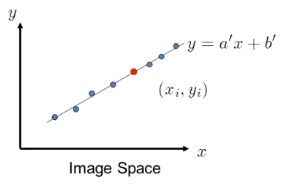
\includegraphics[width=8cm,height=6cm,keepaspectratio]{img/hough.png}
  \caption{set of points belonging to a line}
\end{figure}

The basic procedure of Hough Transform is:
\begin{enumerate}
\item Obtain a binary edge using any edge detection techiniques discussed so far in the report.
\item Quantify $\rho\theta-$ plane.
\item Examine the number of intersects at each cell in the $\rho\theta-$ plane.
\item Bridge the gap based on continuity.
\end{enumerate}

\subsection{Active Contours}\index{Active Contours}
\begin{figure}[h!]
  \centering
  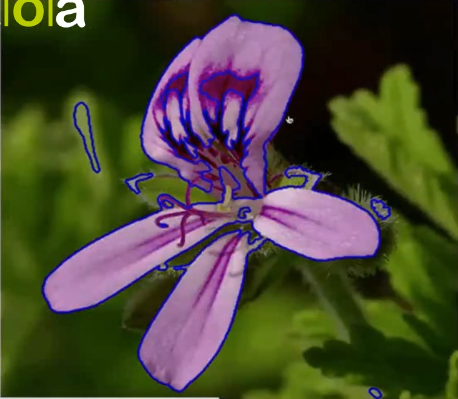
\includegraphics[width=8cm,height=6cm,keepaspectratio]{img/active_contour.png}
  \caption{Active contour in action}
\end{figure}

Active Contours(a.k.a \textbf{snakes}) is an advanced edge-detection techniques. It is a controlled continuity contour like a elastic rubber band which encloses a target object by locking its edges. The initial contour is assigned velocities than move towards the target object boundary of interest.
\\
\\
In the future, we would like to work on applying active contour to all the edge-detection problems. Also, we would apply the hough transform to complete incomplete boundaries of images.
%%% Local Variables:
%%% mode: latex
%%% TeX-master: t
%%% End:

